\documentclass[border=8pt]{standalone}
\usepackage[T1]{fontenc}\usepackage{helvet}\renewcommand{\familydefault}{\sfdefault}
\usepackage{tikz}\usetikzlibrary{arrows.meta, positioning, calc, backgrounds}
\definecolor{ink}{HTML}{1a1916}
\definecolor{inktwo}{HTML}{3a3a35}
\definecolor{inkthree}{HTML}{6a6862}
\definecolor{rule}{HTML}{b8b09a}
\definecolor{amber}{HTML}{a8730a}
\definecolor{red}{HTML}{c8261a}
\definecolor{paper}{HTML}{f0eee5}
\definecolor{slab}{HTML}{d8d4c6}
\tikzset{
  >={Stealth[length=2.2mm]},
  wire/.style={line width=0.8pt, ink},
  modwire/.style={line width=0.6pt, dashed, ink},
  tastewire/.style={line width=0.6pt, dashed, amber},
  gatewire/.style={line width=0.6pt, dotted, ink},
  block/.style={rectangle, draw=ink, line width=0.9pt, fill=slab, minimum width=3.0cm, minimum height=1.9cm, inner sep=0pt},
  perf/.style={rectangle, draw=ink, line width=0.7pt, minimum width=3.0cm, minimum height=0.7cm, inner sep=2pt, font=\footnotesize, text=ink},
  title/.style={font=\scriptsize\bfseries, text=ink, anchor=north, inner sep=2pt},
  jack/.style={circle, draw=ink, fill=paper, line width=0.5pt, minimum size=3.2pt, inner sep=0pt},
  plabel/.style={font=\tiny, text=inktwo, anchor=west, inner sep=1pt},
  olabel/.style={font=\tiny, text=inktwo, anchor=east, inner sep=1pt},
  settings/.style={font=\scriptsize, text=ink, align=left, anchor=north west, inner sep=1pt, text width=2.9cm},
}
\begin{document}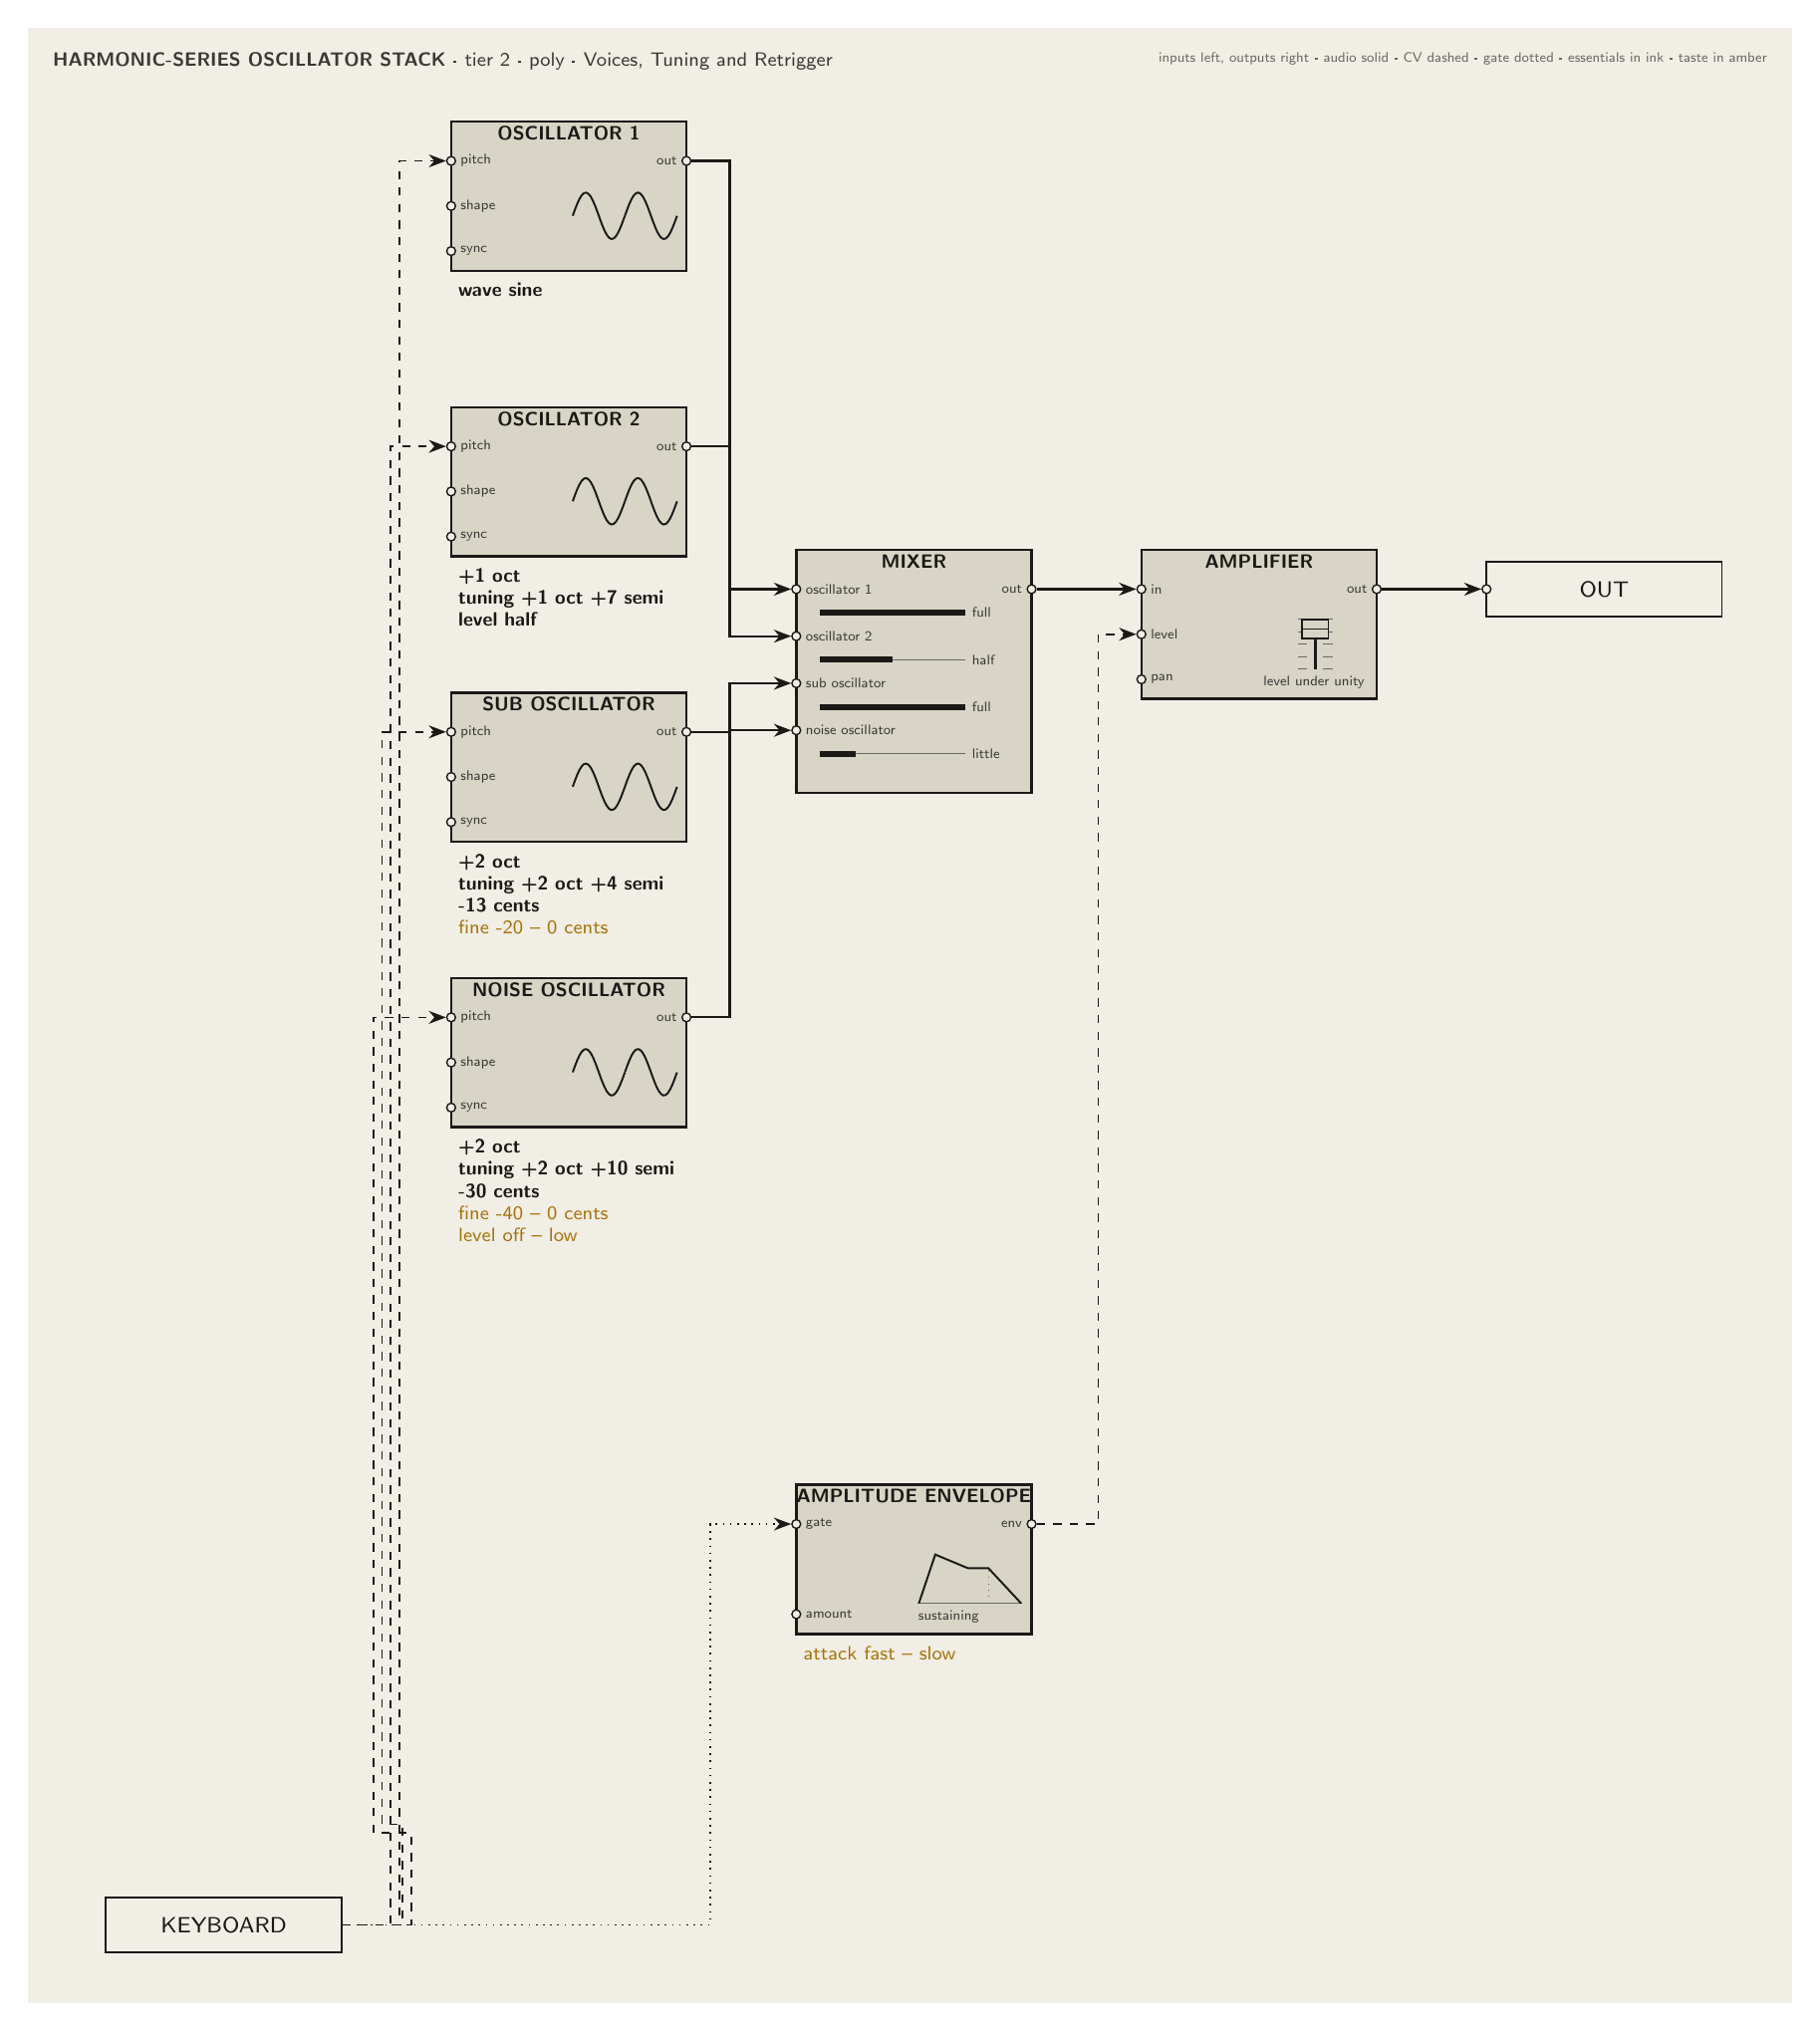
\begin{tikzpicture}
\begin{scope}[on background layer]\fill[paper] (-2.5,-17.58) rectangle (20.0,7.609999999999999);\end{scope}
\node[block, minimum height=1.9cm] (osc1) at (4.4,5.459999999999999) {};
\node[title] at (osc1.north) {OSCILLATOR 1};
\node[jack] (osc1-pitch) at (2.9000000000000004,5.909999999999999) {};
\node[plabel] at (2.9800000000000004,5.909999999999999) {pitch};
\node[jack] (osc1-shape) at (2.9000000000000004,5.334999999999999) {};
\node[plabel] at (2.9800000000000004,5.334999999999999) {shape};
\node[jack] (osc1-sync) at (2.9000000000000004,4.76) {};
\node[plabel] at (2.9800000000000004,4.76) {sync};
\node[jack] (osc1-out) at (5.9,5.909999999999999) {};
\node[olabel] at (5.82,5.909999999999999) {out};
\begin{scope}
\draw[ink, line width=0.7pt] plot[domain=0.000:0.500, samples=24, variable=\u] ({4.450+\u*1.330},{4.840+(0.740)*(0.5+0.4*sin(360*(\u*2))+0.0)});
\draw[ink, line width=0.7pt] plot[domain=0.500:1.000, samples=24, variable=\u] ({4.450+\u*1.330},{4.840+(0.740)*(0.5+0.4*sin(360*(\u*2))+0.0)});
\end{scope}
\node[settings] at (2.95,4.389999999999999) {\textbf{wave sine}};
\node[block, minimum height=1.9cm] (osc2) at (4.4,1.8199999999999998) {};
\node[title] at (osc2.north) {OSCILLATOR 2};
\node[jack] (osc2-pitch) at (2.9000000000000004,2.2699999999999996) {};
\node[plabel] at (2.9800000000000004,2.2699999999999996) {pitch};
\node[jack] (osc2-shape) at (2.9000000000000004,1.6949999999999996) {};
\node[plabel] at (2.9800000000000004,1.6949999999999996) {shape};
\node[jack] (osc2-sync) at (2.9000000000000004,1.1199999999999997) {};
\node[plabel] at (2.9800000000000004,1.1199999999999997) {sync};
\node[jack] (osc2-out) at (5.9,2.2699999999999996) {};
\node[olabel] at (5.82,2.2699999999999996) {out};
\begin{scope}
\draw[ink, line width=0.7pt] plot[domain=0.000:0.500, samples=24, variable=\u] ({4.450+\u*1.330},{1.200+(0.740)*(0.5+0.4*sin(360*(\u*2))+0.0)});
\draw[ink, line width=0.7pt] plot[domain=0.500:1.000, samples=24, variable=\u] ({4.450+\u*1.330},{1.200+(0.740)*(0.5+0.4*sin(360*(\u*2))+0.0)});
\end{scope}
\node[settings] at (2.95,0.7499999999999999) {\textbf{+1 oct} \\ \textbf{tuning +1 oct +7 semi} \\ \textbf{level half}};
\node[block, minimum height=1.9cm] (sub) at (4.4,-1.8199999999999998) {};
\node[title] at (sub.north) {SUB OSCILLATOR};
\node[jack] (sub-pitch) at (2.9000000000000004,-1.3699999999999999) {};
\node[plabel] at (2.9800000000000004,-1.3699999999999999) {pitch};
\node[jack] (sub-shape) at (2.9000000000000004,-1.9449999999999998) {};
\node[plabel] at (2.9800000000000004,-1.9449999999999998) {shape};
\node[jack] (sub-sync) at (2.9000000000000004,-2.5199999999999996) {};
\node[plabel] at (2.9800000000000004,-2.5199999999999996) {sync};
\node[jack] (sub-out) at (5.9,-1.3699999999999999) {};
\node[olabel] at (5.82,-1.3699999999999999) {out};
\begin{scope}
\draw[ink, line width=0.7pt] plot[domain=0.000:0.500, samples=24, variable=\u] ({4.450+\u*1.330},{-2.440+(0.740)*(0.5+0.4*sin(360*(\u*2))+0.0)});
\draw[ink, line width=0.7pt] plot[domain=0.500:1.000, samples=24, variable=\u] ({4.450+\u*1.330},{-2.440+(0.740)*(0.5+0.4*sin(360*(\u*2))+0.0)});
\end{scope}
\node[settings] at (2.95,-2.8899999999999997) {\textbf{+2 oct} \\ \textbf{tuning +2 oct +4 semi -13 cents} \\ \textcolor{amber}{fine -20 -- 0 cents}};
\node[block, minimum height=1.9cm] (noise) at (4.4,-5.459999999999999) {};
\node[title] at (noise.north) {NOISE OSCILLATOR};
\node[jack] (noise-pitch) at (2.9000000000000004,-5.009999999999999) {};
\node[plabel] at (2.9800000000000004,-5.009999999999999) {pitch};
\node[jack] (noise-shape) at (2.9000000000000004,-5.584999999999999) {};
\node[plabel] at (2.9800000000000004,-5.584999999999999) {shape};
\node[jack] (noise-sync) at (2.9000000000000004,-6.159999999999998) {};
\node[plabel] at (2.9800000000000004,-6.159999999999998) {sync};
\node[jack] (noise-out) at (5.9,-5.009999999999999) {};
\node[olabel] at (5.82,-5.009999999999999) {out};
\begin{scope}
\draw[ink, line width=0.7pt] plot[domain=0.000:0.500, samples=24, variable=\u] ({4.450+\u*1.330},{-6.080+(0.740)*(0.5+0.4*sin(360*(\u*2))+0.0)});
\draw[ink, line width=0.7pt] plot[domain=0.500:1.000, samples=24, variable=\u] ({4.450+\u*1.330},{-6.080+(0.740)*(0.5+0.4*sin(360*(\u*2))+0.0)});
\end{scope}
\node[settings] at (2.95,-6.529999999999999) {\textbf{+2 oct} \\ \textbf{tuning +2 oct +10 semi -30 cents} \\ \textcolor{amber}{fine -40 -- 0 cents} \\ \textcolor{amber}{level off -- low}};
\node[block, minimum height=3.1cm] (mix) at (8.8,-0.6000000000000001) {};
\node[title] at (mix.north) {MIXER};
\node[jack] (mix-osc1) at (7.300000000000001,0.44999999999999996) {};
\node[plabel] at (7.380000000000001,0.44999999999999996) {oscillator 1};
\draw[inkthree, line width=0.3pt] (7.600,0.150) -- (9.450,0.150);
\draw[ink, line width=2.2pt] (7.600,0.150) -- (9.450,0.150);
\node[font=\tiny, text=inktwo, anchor=west, inner sep=1pt] at (9.500,0.150) {full};
\node[jack] (mix-osc2) at (7.300000000000001,-0.15000000000000002) {};
\node[plabel] at (7.380000000000001,-0.15000000000000002) {oscillator 2};
\draw[inkthree, line width=0.3pt] (7.600,-0.450) -- (9.450,-0.450);
\draw[ink, line width=2.2pt] (7.600,-0.450) -- (8.525,-0.450);
\node[font=\tiny, text=inktwo, anchor=west, inner sep=1pt] at (9.500,-0.450) {half};
\node[jack] (mix-sub) at (7.300000000000001,-0.75) {};
\node[plabel] at (7.380000000000001,-0.75) {sub oscillator};
\draw[inkthree, line width=0.3pt] (7.600,-1.050) -- (9.450,-1.050);
\draw[ink, line width=2.2pt] (7.600,-1.050) -- (9.450,-1.050);
\node[font=\tiny, text=inktwo, anchor=west, inner sep=1pt] at (9.500,-1.050) {full};
\node[jack] (mix-noise) at (7.300000000000001,-1.3499999999999999) {};
\node[plabel] at (7.380000000000001,-1.3499999999999999) {noise oscillator};
\draw[inkthree, line width=0.3pt] (7.600,-1.650) -- (9.450,-1.650);
\draw[ink, line width=2.2pt] (7.600,-1.650) -- (8.062,-1.650);
\node[font=\tiny, text=inktwo, anchor=west, inner sep=1pt] at (9.500,-1.650) {little};
\node[jack] (mix-out) at (10.3,0.44999999999999996) {};
\node[olabel] at (10.22,0.44999999999999996) {out};
\node[block, minimum height=1.9cm] (amp) at (13.200000000000001,0.0) {};
\node[title] at (amp.north) {AMPLIFIER};
\node[jack] (amp-in) at (11.700000000000001,0.44999999999999996) {};
\node[plabel] at (11.780000000000001,0.44999999999999996) {in};
\node[jack] (amp-level) at (11.700000000000001,-0.125) {};
\node[plabel] at (11.780000000000001,-0.125) {level};
\node[jack] (amp-pan) at (11.700000000000001,-0.7) {};
\node[plabel] at (11.780000000000001,-0.7) {pan};
\node[jack] (amp-out) at (14.700000000000001,0.44999999999999996) {};
\node[olabel] at (14.620000000000001,0.44999999999999996) {out};
\begin{scope}
\draw[ink, line width=1.2pt] (13.915,-0.570) -- (13.915,0.070);
\draw[inkthree, line width=0.3pt] (13.695,-0.570) -- (13.815,-0.570) (14.015,-0.570) -- (14.135,-0.570);
\draw[inkthree, line width=0.3pt] (13.695,-0.410) -- (13.815,-0.410) (14.015,-0.410) -- (14.135,-0.410);
\draw[inkthree, line width=0.3pt] (13.695,-0.250) -- (13.815,-0.250) (14.015,-0.250) -- (14.135,-0.250);
\draw[inkthree, line width=0.3pt] (13.695,-0.090) -- (13.815,-0.090) (14.015,-0.090) -- (14.135,-0.090);
\draw[inkthree, line width=0.3pt] (13.695,0.070) -- (13.815,0.070) (14.015,0.070) -- (14.135,0.070);
\fill[slab, draw=ink, line width=0.6pt] (13.745,-0.178) rectangle (14.085,0.062);
\draw[ink, line width=0.5pt] (13.745,-0.058) -- (14.085,-0.058);
\node[font=\tiny, text=inktwo, anchor=north west, inner sep=0pt] at (13.250,-0.650) {level under unity};
\end{scope}
\node[block, minimum height=1.9cm] (aenv) at (8.8,-11.919999999999998) {};
\node[title] at (aenv.north) {AMPLITUDE ENVELOPE};
\node[jack] (aenv-gate) at (7.300000000000001,-11.469999999999999) {};
\node[plabel] at (7.380000000000001,-11.469999999999999) {gate};
\node[jack] (aenv-amount) at (7.300000000000001,-12.62) {};
\node[plabel] at (7.380000000000001,-12.62) {amount};
\node[jack] (aenv-out) at (10.3,-11.469999999999999) {};
\node[olabel] at (10.22,-11.469999999999999) {env};
\begin{scope}
\draw[inkthree, line width=0.3pt] (8.850,-12.481) -- (10.180,-12.481);
\draw[ink, line width=0.7pt] (8.863,-12.481) -- (9.072,-11.859) -- (9.489,-12.033) -- (9.750,-12.033) -- (10.167,-12.481);
\draw[inkthree, line width=0.3pt, dotted] (9.750,-12.481) -- (9.750,-12.033);
\node[font=\tiny, text=inktwo, anchor=north west, inner sep=0pt] at (8.850,-12.570) {sustaining};
\end{scope}
\node[settings] at (7.3500000000000005,-12.989999999999997) {\textcolor{amber}{attack fast -- slow}};
\node[perf] (key) at (0.0,-16.58) {KEYBOARD};
\node[perf, fill=paper] (out) at (17.6,0.44999999999999996) {OUT}; \node[jack] (out-in) at (16.1,0.44999999999999996) {};
\draw[wire,->] (osc1-out) -- (6.45,5.909999999999999) |- (mix-osc1);
\draw[wire,->] (osc2-out) -- (6.45,2.2699999999999996) |- (mix-osc2);
\draw[wire,->] (sub-out) -- (6.45,-1.3699999999999999) |- (mix-sub);
\draw[wire,->] (noise-out) -- (6.45,-5.009999999999999) |- (mix-noise);
\draw[wire,->] (mix-out) -- (10.850000000000001,0.44999999999999996) |- (amp-in);
\draw[wire,->] (amp-out) -- (out-in);
\draw[modwire,->] (aenv-out) -- (11.15,-11.469999999999999) -- (11.15,-0.125) -- (amp-level);
\draw[modwire,->] (key.east) -- (2.2400000000000007,-16.58) -- (2.2400000000000007,5.909999999999999) -- (osc1-pitch);
\draw[modwire,->] (key.east) -- (2.1300000000000003,-16.58) -- (2.1300000000000003,2.2699999999999996) -- (osc2-pitch);
\draw[modwire,->] (key.east) -- (2.28,-16.58) -- (2.28,-15.299999999999997) -- (2.0200000000000005,-15.299999999999997) -- (2.0200000000000005,-1.3699999999999999) -- (sub-pitch);
\draw[modwire,->] (key.east) -- (2.39,-16.58) -- (2.39,-15.409999999999997) -- (1.9100000000000006,-15.409999999999997) -- (1.9100000000000006,-5.009999999999999) -- (noise-pitch);
\draw[gatewire,->] (key.east) -- (6.200000000000001,-16.58) -- (6.200000000000001,-11.469999999999999) -- (aenv-gate);
\node[anchor=north west, font=\scriptsize, text=inktwo] at (-2.3,7.409999999999999) {\textbf{HARMONIC-SERIES OSCILLATOR STACK} · tier 2 · poly · Voices, Tuning and Retrigger};
\node[anchor=north east, font=\tiny, text=inkthree] at (19.8,7.409999999999999) {inputs left, outputs right · audio solid · CV dashed · gate dotted · essentials in ink · taste in amber};
\end{tikzpicture}\end{document}
